% !TEX root = /home/frank/School/thesis_text/thesis.tex



\chapter{platform overview}

This device integrates a dual core ARM Cortex-A9 and Xilinx Programmable Logic in a single device. The communication between these two components goes through an ARM AMBA AXI 4 bus. Each processor also has a single/double precision floating point extension. An overview of the architecture of the Zynq processor is given in the figure below.[22]

\begin{figure}[H]
\centering
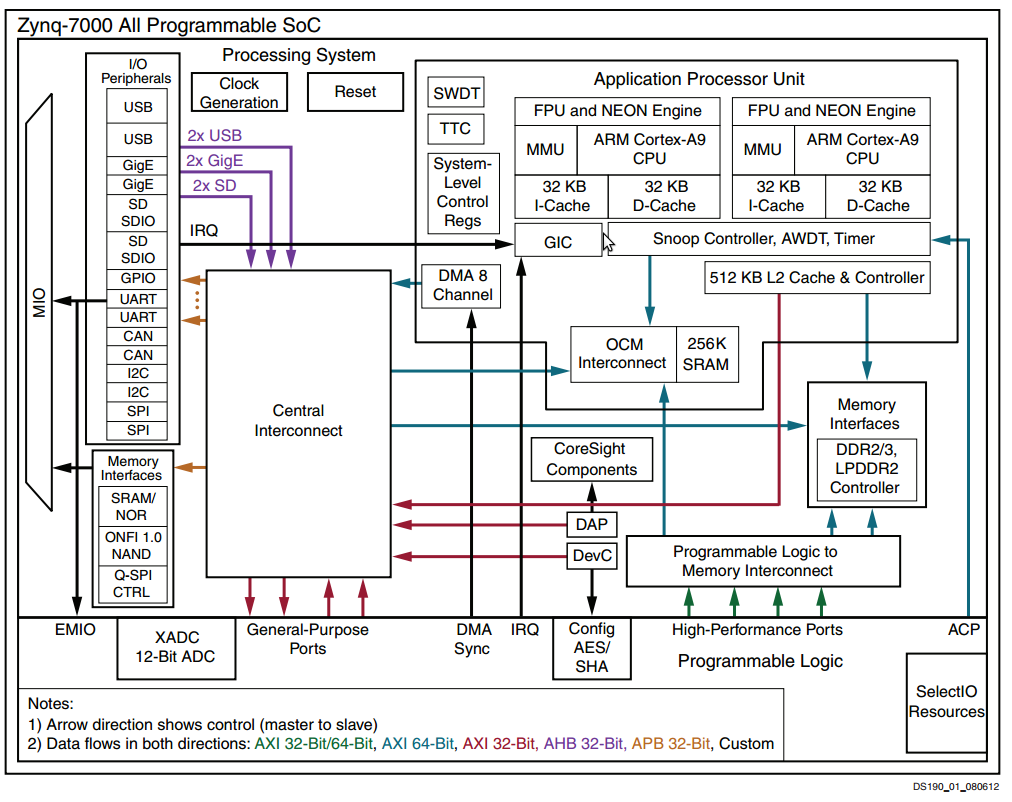
\includegraphics[scale=0.35]{/home/frank/School/thesis_text/images/zynq_overview.png}
\caption{Zynq -7000 SoC overview}
\label{img:zynq_overview}
\end{figure}


The Advanced Microcontroller Bus Architecture (AMBA) is an open standard specification for a bus system used in SoCs to interconnect and manage different functional blocks. The AXI specification which is part of AMBA is targeted at high performance, high frequency systems. The Achilles' heel of HPC is usually costly communications. It would be interesting to research the performance of an on-chip interconnect system and a typical PCIe bus.Due to the recent launch of the zynq-7000 architecture there is little to no academic information to be found about it.\\
Profiling for this platform is done through the Xilinx SDK software. It needs to be noted that the profiler cannot profile the hardware implemented in the programmable logic. For this other tools have to be used.[23]\\
The board which will be used for this implementation is the Xilinx ZC702 which contains the XC7Z020 CLG484-1 AP SoC combined with the Video and Imaging kit. This contains a high definition camera and the necessary board to interface it with the SoC.

